\section{Simulation}
\label{sec:simulation}

In this section, we investigate how to simulate future paths of the time series $y_t$. 
%We use this model to produce $K$ future values for the time serie $y_t$. 
Let $T$ be the total number of observations of $y_t$. We produce $S$ different paths with size $K$ for each. 
We have $T$ observations of $y_t$ and we want to simulate  Given a vector of explanatory variables $x_t$, let $q_t^\alpha$ be given by the following linear model:
\begin{equation}
q_t^\alpha = \beta_0^\alpha +  x_t^T \beta^\alpha + \varepsilon_t,
\label{eq:fun-quantile}
\end{equation}
where $\beta^\alpha$ is a vector of coefficients for the explanatory variables. The variables chosen to compose $x_t$ can be either exogenous variables, autoregressive components of $y_t$ or both. As the distribution of $\varepsilon_t$ is unknown, we have to use a nonparametric approach in order to estimate its one-step ahead density.

The coefficients $\beta_0^\alpha$ and $\beta^\alpha$ are the solution of the minimization problem given in equation \ref{eq:qar-lp}, reproduced here for convenience:
\begin{equation}
\begin{aligned}\min_{\beta_0,\beta,\varepsilon_{t}^{+},\varepsilon_{t}^{-}} & \sum_{t=1}^{n}\left(\alpha\varepsilon_{t}^{+}+(1-\alpha)\varepsilon_{t}^{-}\right)\\
\mbox{s.t. } & \varepsilon_{t}^{+}-\varepsilon_{t}^{-}=y_{t} - \beta_0 - \beta^T x_{t},\qquad\forall t\in\{1,\dots,n\},\\
& \varepsilon_t^+,\varepsilon_t^- \geq 0, \qquad \forall t \in \{1,\dots,n\}.
\end{aligned}
\label{eq:problem-quantile-regression}
\end{equation}

To produce $S$ different paths of $\{ \hat{y}_t \}_{t=T+1}^{T+K}$, we use the following procedure:

\noindent\rule{\textwidth}{3pt}

Procedure for simulating $S$ scenarios of $y_t$

\noindent\rule{\textwidth}{1pt}

\begin{enumerate}
	

\item For every quantile $\alpha_i \in (0,1)$, we use equation \ref{eq:fun-quantile} to produce a forecast of $\hat{q}^{\alpha_i}_{T+1}$, as $x_{T+1}$ is supposed to be known at time $T+1$. In the presence of exogenous variables that are unknown, it is advisable to incorporate its uncertainty by considering different scenarios. In each scenario, though, $x_{T+1}$ must be considered fully known. 

\item In any given $t$, by choosing many different values of $\alpha_i$, we can estimate a sequence of quantiles $q^{\alpha_1}_{t} \leq q^{\alpha_2}_{t} \leq \dots \leq q^{\alpha_Q}_{t}$ with $0 < \alpha_1 < \alpha_2 < \dots < \alpha_Q < 1$. 
Let $F_{y_{T+1}}$ be the estimated distribution function of ${y}_{T+1}$. 
The process of fitting $\hat{F}_{y_{T+1}}$ is by mapping every $\alpha_i$ with its estimated quantile $\hat{q}^{\alpha_i}$. A problem arises for the distribution extremities, because when $\alpha = 0$ or $\alpha = 1$, the problem \ref{eq:problem-quantile-regression} becomes unbounded.
In order to find good estimates for $y_{T+1}$ when $F_{y_{T+1}}$ approaches 0 or 1, we can either use a kernel smoothing function, splines, linear approximation, or any other method. 
\textbf{This will be developed later.}
When this sequence of chosen $\alpha_i$ is thin enough, we can approximate well the distribution function of $y_{T+1}$, as is shown in Figure \ref{fig:grafico-quantis}. 
Thus, the distribution found for $\hat{y}_{T+1}$ is nonparametric, as no previous assumptions are made about its shape, and its form is fully recovered by the data we have.

\begin{figure}[h]
\centering
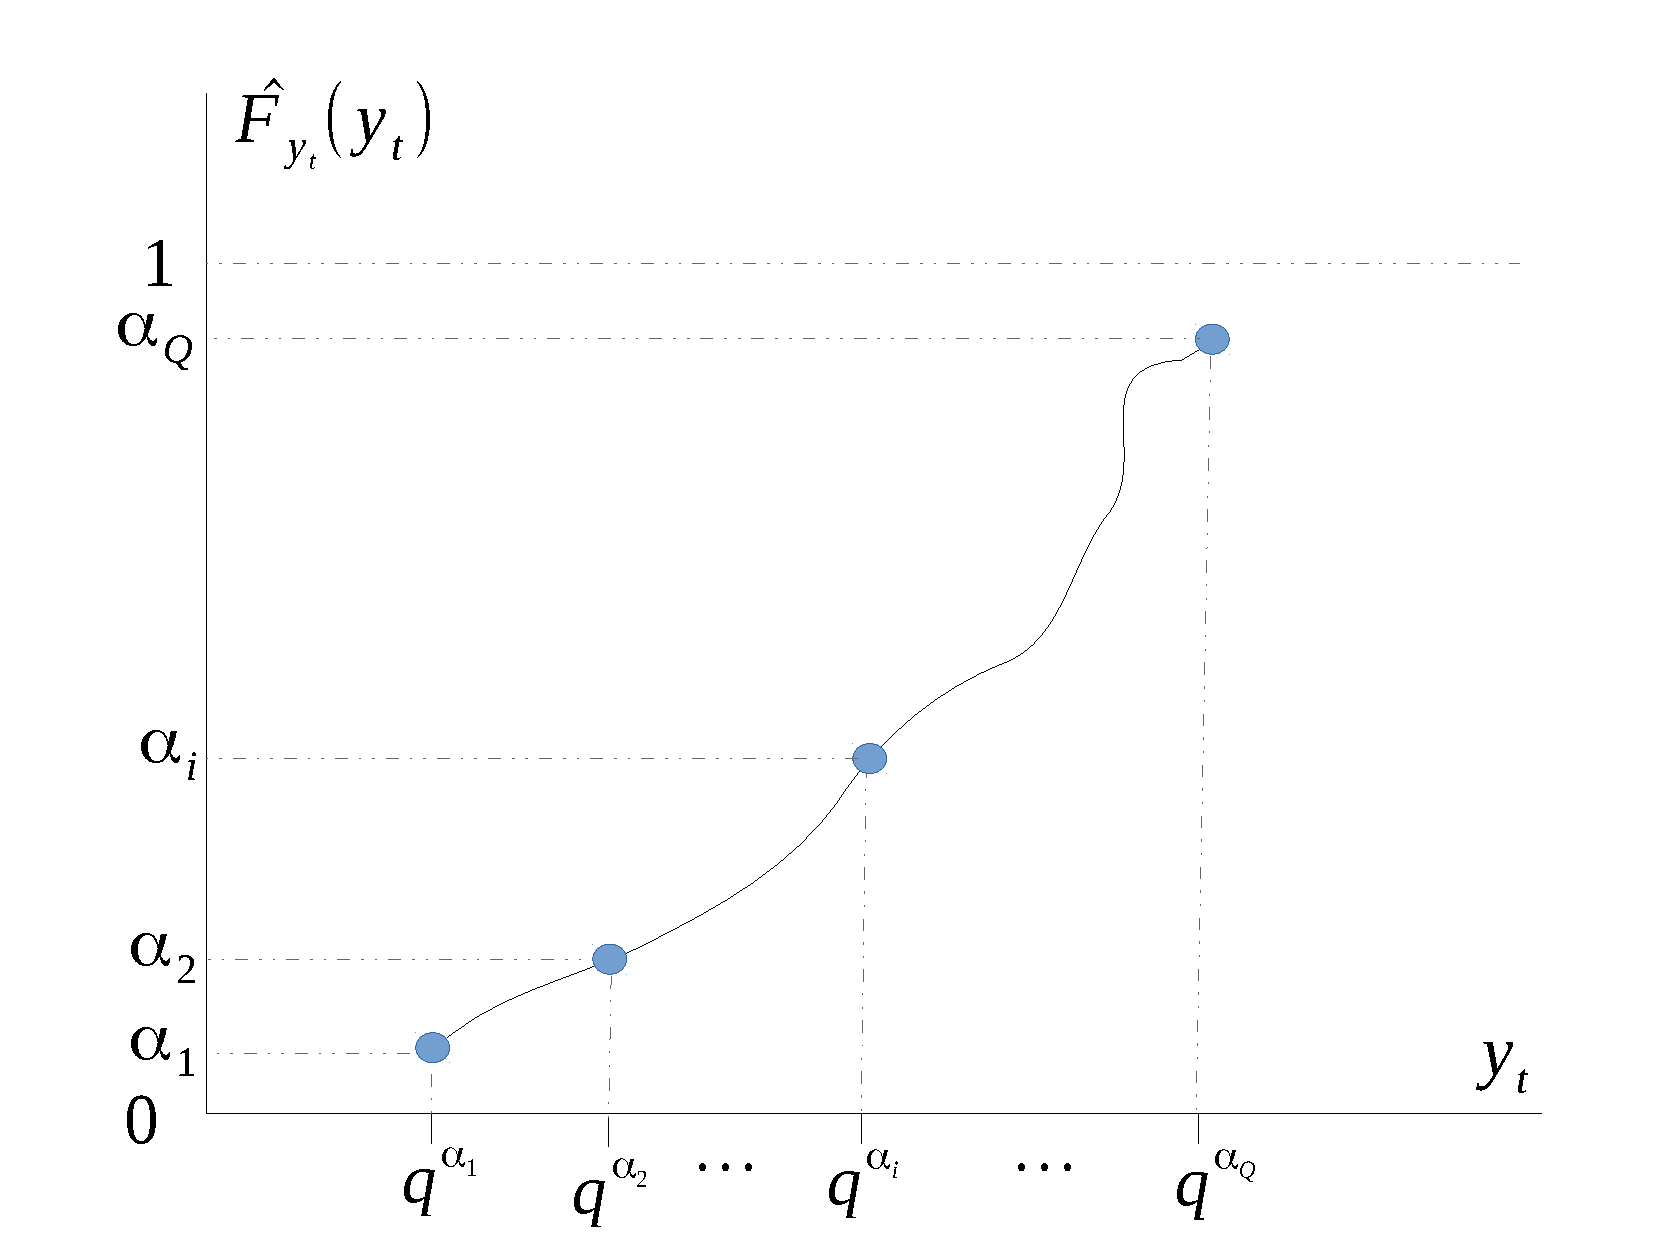
\includegraphics[width=0.7\linewidth]{./Figuras/grafico-quantis}
\caption{Fitting a distribution function from quantile estimations}
\label{fig:grafico-quantis}
\end{figure}


\item Once we have a distribution for $y_{T+1}$, we can generate $S$ different simulated values, drawn from the distribution $\hat{F}_{y_{T+1}}$ found on step 2. 
Let $X$ be a random variable with uniform distribution over the interval $[0,1]$. By using results from the Probability Integral Transform, we know that the random variable $F^{-1}_{y_{T+1}}(X)$ has the same distribution as $y_{T+1}$. So, by drawing a sample of size $S$ from $X$ and applying the inverse function of $F_{y_{T+1}}$, we have our sample of size $K$ for $y_{T+1}$.

\item Each one of the $S$ different values for $y_{T+1}$ will be the starting point of a different path. Now, for each $t \in [T+2,T+K]$ and $s \in S$, we have to estimate the quantiles $q_{t,s}^{\alpha_i}$ and find a distribution function for $\hat{F}_{y_{t,s}}$ just like it was done on step 2.
Note that when $t > T+2$, every estimate will be scenario dependent, hence there will be $S$ distribution functions estimated for each period $t$. From now on, in each path just one new value will be drawn randomly from the one-step ahead distribution function - as opposed to what was carried on step 3, when $S$ values were simulated. As there will be $S$ distribution functions - one for each path, in each period $t$ it will be produced exact $S$ values for $y_t$, one for its own path. Repeating this step until all values of $t$ and $s$ are simulated will give us the full simulations that we are looking for.
\end{enumerate}


\noindent\rule{\textwidth}{1pt}